\setchapterimage[8.5cm]{results/branimage002}
\setchapterpreamble[u]{\margintoc}
\chapter{Stacking Analyses with IceCube}
\labch{results}
\begin{fquote}[Oscar Wilde][Lady Windermere's Fan][1893]We are all in the gutter, but some of us are looking at the stars
\end{fquote}
   
A key component of this thesis is the application of the unbinned likelihood analysis method outlined in Chapter \ref{ch:llh} to specific astrophysical objects, to test for correlations indicating neutrino emission. The outcomes of these tests were then analysed in the context of diffuse neutrino flux arising from astrophysical populations, following the framework introduced in Chapter \ref{ch:neutrino_cosmology}. All results are outlined below.

All calculations were  performed using the \emph{\href{https://github.com/IceCubeOpenSource/flarestack}{Flarestack}} code, developed by the author. Some results presented were previously published in proceedings written by the author \sidecite{icrc_tde}.

\section{Tidal Disruption Events}

One novel result of this thesis is a stacking analysis of Tidal Disruption Events (TDEs) (see Chapter \ref{ch:sources}), the first such experimental search for a TDE-neutrino correlation. The details of this analysis are outlined below.

\subsection*{Signal Hypothesis}

As outlined Chapter \ref{ch:sources}, theoretical modelling of neutrino emission in TDEs generally distinguishes between those with relativistic jets and those without. In recognition of this, we ultimately have two distinct hypotheses to test:

\begin{enumerate}
	\item Neutrino emission from on-axis relativistic jets
	\item Neutrino emission from other mechanisms
\end{enumerate}

The timescales predicted for neutrino emission have varied substantially. In general, neutrino emission is expected to occur close to the peak EM brightness of the flare, with durations of a few hours to $\sim$ 100 days. There are no scenarios for neutrino emission preceding disruption. 

\subsection*{Catalogue Compilation}

To perform a correlation analysis, a list of sources must first be compiled. One list of TDEs is maintained by the \emph{\href{https://tde.space/}{OpenTDECatalog}} \sidecite{tde_catalog_paper}, containing relevant metadata and photometry. The database prioritises completeness by containing all objects with a possible TDE classification, even when those classifications are ambiguous \cite{tde_catalog_paper}, and will thus by construction suffer from source contamination. The database itself is maintained by volunteers, and is thus not entirely complete. For the compilation of a catalogue for this thesis, the list from the \emph{\href{https://tde.space/}{OpenTDECatalog}} was supplemented by additional objects and data from the literature.

At the time of catalogue compilation in 2018, this database contained approximately 70 objects. Of these, 3 had clear evidence of on-axis relativistic jets, while the remaining 67 did not. We further exclude those objects with peaks >100 days before the start of data-taking during the IC40 data season on 4th May 2008 (see Chapter \ref{ch:icecube}), as these objects did not overlap our neutrino dataset. We are left with 53 TDEs for correlation.

From the starting point of all TDEs, one distinct subsample was created:

\begin{itemize}
	\item \textbf{Jetted TDEs} are X-Ray-bright TDEs which launched relativistic jets pointing towards the Earth. There are three jetted TDEs, and neutrino emission is most promising from this category
\end{itemize}

These three jetted TDEs share similar properties, namely that they were all sufficiently bright to be discovered serendipitously by observations of the \textit{Swift}-BAT X-ray telescope. They each have well-sampled lightcurves, with the time of jet-launching constrained to a window of a few days. Given the consistent observational features of luminous, hard X-ray emission which rapidly fades, it is likely that all three objects are indeed jetted TDEs. The jetted TDEs were used to test Hypothesis 1.

Hypothesis 2 could then be tested with the remaining ``non-jetted'' TDEs, defined as those TDEs without on-axis relativistic jets. These non-jetted TDEs form an observationally-distinct class of objects. They may have off-axis relativistic jets, or mildly relativistic outflows, but none exhibit the characteristic hard X-ray emission associated with on-axis relativistic jets .

Beyond this, the properties of non-jetted TDEs are highly heterogeneous. They are discovered across a range of wavelengths (e.g soft x-ray, optical, IR) with varying multi-wavelength coverage. There are a handful of compelling TDE candidates, often with comprehensive multi-epoch spectroscopic observations, for which alternative explanations are disfavoured. However, in the vast majority of cases, a definite classification cannot be made. To avoid contamination from misclassified objects, primarily AGN or SN, a clean \emph{golden sample} was defined consisting `reliably-classified' TDEs. These were judged primarily based on their uncontested classification in the literature, and were typically charecterised by multiple epochs of spectroscopic coverage and contemporaneous multi-wavenlegth coverage:

\begin{itemize}
	\item \textbf{Golden TDEs} are strong candidates where the TDE interpretation is supported by multiple spectra
\end{itemize}

The remaining objects are then candidate TDEs, with a possible but not definitive classification. 

There is one distinct subclass of candidates containing flares observed in dusty galaxies via IR emission \sidecite{wang_mir_tdes_2018}. One possible explanation is that the flares arise from a dust-obscured TDE, with the dust then slowly reprocessing the electromagnetic radiation from the galaxy core.  For such reprocessing, there would be a time delay between the disruption itself and the corresponding IR flare. Because we expect that neutrinos should begin soon after disruption, the timescale for neutrino emission from obscured TDEs would have significant additional uncertainty. 

We thus treat these candidate \emph{obscured TDEs} separately from the other candidate TDEs:

\begin{itemize}
		\item \textbf{Obscured TDEs} are TDE candidates which occur in very dusty galaxies, and are only observed via reprocessed infra-red emission. 
	\item \textbf{Silver TDEs} are all other candidates, where a TDE interpretation is either likely or not disfavoured.
\end{itemize}

All catalogues are summarised in Table \ref{tab:stacking_cat}, with full details provided in the Appendix (Chapter \ref{ch:catalogues}).

\begin{table*}[]
	\centering
	\begin{tabular}{||c c c c |} 
		\hline
		Catalogue & Source Class & Size & Description \\ [0.5ex] 
		\hline\hline
		Jetted & Jetted TDEs &  3 & \textit{Probable TDEs with on-axis jets}\\ 
		\hline
		Golden & Non-Jetted TDEs & 13 & \textit{Probable TDEs with convincing classification}\\
		\hline
		Silver & Non-Jetted TDEs & 24 & \textit{Candidate TDEs with ambiguous classification}\\
		\hline
		Obscured & Non-Jetted TDEs & 13 & \textit{Candidate TDEs in dusty galaxies}\\[1ex] 
		\hline
	\end{tabular}
	\caption{Summary of the four TDE catalogues..}
	\label{tab:stacking_cat}
\end{table*}{}

\subsection*{Search Windows}

To account for the heterogeneous datasets, an individual search window was defined for each TDE, with the aim for identifying the period of peak electromagnetic emission. For jetted/gold/silver TDE, the following criteria were used:

\begin{itemize}
	\item For TDEs in which the light curve was observed when rising, the first detection is taken as the window start.
	
	\item For TDEs without an observation during lightcurve rise, the last upper limit is taken as the window start.
	
	\item The maximum date was taken as the date on which the brightest TDE luminosity measurement was performed.
	
	\item The window extends from the defined window start to 100 days after the maximum date
	
\end{itemize}

Applying these criteria gives a tailored search window for each TDE. Obscured TDEs instead had a search window extending from 300 days before peak to 100 days after peak, to account for potential delay following neutrino emission. The search window for each source is provided in Appendix Chapter \ref{ch:catalogues}. It is the first such catalogue to contain time windows, and could also be used for stacking analyses of e.g gamma-ray emission.

\subsection*{Analysis and Results}

As outlined in Chapter \ref{ch:llh}, a standard \emph{stacking analysis} requires an additional assumption on the expected relative neutrino emission of each source in a catalogue. However, these TDE catalogues are characterised by small numbers of heterogeneous sources. With a mix of observation cadences and multi-wavelength coverage, there is no obvious proxy for neutrino emission. There is no evidence of standard-candle behaviour in EM wavelengths, so there is no reason to think it would hold for neutrino emission. We are left with no clear method to predict the relative contributions, and for this reason, an agnostic approach is instead applied. Using the method outlined in Section \ref{sec:fit_weights}, we fit the contribution of each source in the catalogue individually, requiring only that they share a common neutrino spectrum.

Following the procedure in Chapter \ref{ch:llh}, we perform an unbinned likelihood analysis to obtain results for each catalogue, with fit parameters TS, $\gamma$ and a number of signal events for each source ($n_{k}$). We also obtain a final Test Statistic (TS) value, and calculate a p-value for this TS using pseudotrials. Table \ref{tab:stacking_tests} summarises the results for each catalogue, including $n_{s} = \sum n_{k}$. The individual $n_{k}$ values are provided in the Appendix Chapter \ref{ch:catalogues}.

\begin{table}[]
	\centering
	\begin{tabular}{||c c c| c c c | c||} 
		\hline
		Catalogue & Source Class & Size & $n_{s}$  & $\gamma$ & TS & Pre-trial p-value\\
		\hline\hline
		Jetted & Jetted &  3 & 1.5& 4.0&0.8&0.40\\ 
		\hline
		Golden & Non-Jetted & 13 &3.9&2.4& 2.4&1.00\\
		\hline
		Silver & Non-Jetted & 24 &15.6&2.7&7.9 & 1.00\\
		\hline
		Obscured & Non-Jetted & 13 &29.4&2.8&14.8& 0.04\\[1ex] 
		\hline
	\end{tabular}
	\caption{Summary of results for the four TDE catalogues.}
	\label{tab:stacking_tests}
\end{table}{}

There was no significant correlation identified for any of the catalogues. While the Obscured TDE catalogue yielded the most significant pre-trial p-value, after trial correction using Equation \ref{eq:trial_correction} this is reduced to a value of $p_{\textup{post-trial}}$=0.15, and is thus consistent with background expectations. No discovery of neutrino emission from TDEs is claimed, and \emph{we do not reject the null hypothesis that TDEs and neutrinos are uncorrelated}.

\subsection*{Catalogue limits}

Being unable to reject the null hypothesis, we can instead set an upper limit on neutrino emission, by ruling out scenarios for which we would have expected to reject the null hypothesis. We follow the procedure outlined in Section \ref{sec:sens_uls} to set an upper limit, at 90\% confidence, using pseudoexperiements with simulated signal. In common with most IceCube studies, these limits are only valid \emph{under the assumption that the signal looks like the baseline IceCube MC}, and thus that \emph{the impact of all systematic effects are negligible}.

While our search results in Table \ref{tab:stacking_tests} are agnostic to the relative neutrino contribution of each source, any pseudoexperiments involving simulated signal must make an assumption regarding the intrinsic neutrino luminosity of each source. Though it remains a poor approximation for EM emission, we inject neutrinos under \emph{the assumption that each catalogue source emits the same number of neutrinos according to the same intrinsic energy spectrum}, i.e that TDEs are neutrino standard candles. The corresponding flux on Earth is thus proportional to the inverse distance squared of each source. This flux is injected uniformly across the search windows for each source, as defined in Appendix (Chapter \ref{ch:catalogues}). To conserve energy, the flux-per-source is then inversely proportional to the length of the search window. 

All limits derived below are only valid in the case that all of these assumptions are true. Upper limits are derived for combined neutrino+anti-neutrino emission under the \emph{assumption of an unbroken neutrino power law, between 100 GeV and 10 PeV}, for a variety of spectral limits. These upper limits are shown in Figure \ref{fig:cat_upper_limit_fluence}, in units of integrated neutrino+anti-neutrino fluence for the entire catalogue. 

\begin{figure}[!ht]
	\centering 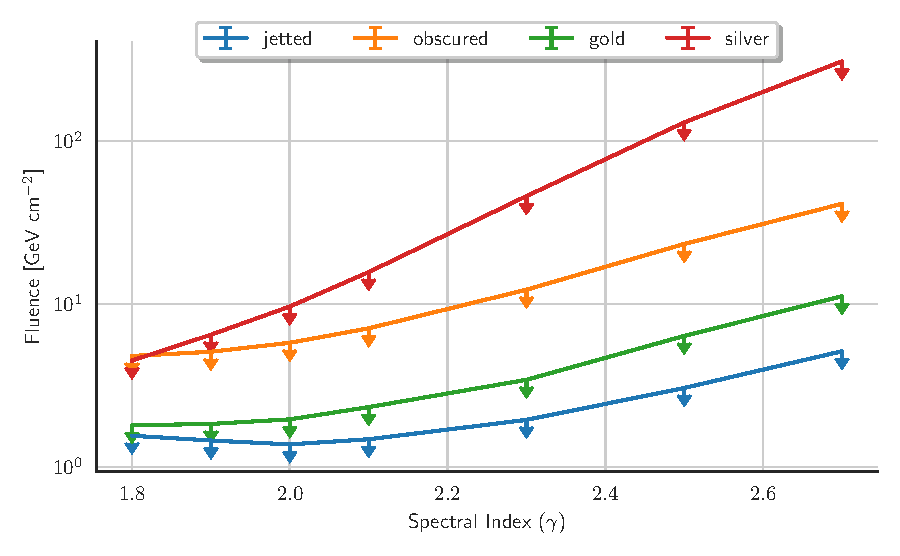
\includegraphics{results/catalogue_limits_fluence}
	\caption{Limits on the neutrino fluence for each catalogue.}
	\label{fig:cat_upper_limit_fluence}
\end{figure}

If Figure \ref{fig:cat_upper_limit_fluence} is contrasted with the time-integrated point source sensitivity (seen in Figure \ref{fig:10yr_ps}), it is clear that the upper limits are substantially higher than the sensitivity for a single source in ten years of data. This is however expected, as a consequence of the additional background that comes with stacking multiple sources. The limits are ranked in order of ascending catalogue size, with the 3-source jetted catalogue being the most stringent and the 24-source silver catalogue being the weakest. The obscured catalogue has a somewhat weaker limit than expected, in notable contrast to the equally-sized gold catalogue, because the former demonstrated a relatively large neutrino excess. 

We can convert these to limits on the integrated neutrino+anti-neutrino per-flavour energy for each source, as shown in Figure \ref{fig:cat_upper_limit}. There is substantially more variation in the scale of these limits, driven by the typical distance scale of the nearest sources in each catalogue (see Appendix Chapter \ref{ch:catalogues}). For the Jetted TDEs, the nearest source lies at $\sim$2000 Mpc , while for silver catalogue the nearest source lies at $\sim$2 Mpc, explaining the dramatic variation in limits between catalogues. All these intrinsic energies are presented as \emph{isotropic-equivalent}, and thus quoted assuming that the emission is emitted isotropically. This is of particular relevance for the Jetted TDEs, for which emission is likely to be highly beamed. As the exact beaming angle is unclear, it is conventional to present such isotropic-equivalent values for comparison, with the true energy likely to be somewhat lower. 

\begin{figure}[!ht]
	\centering 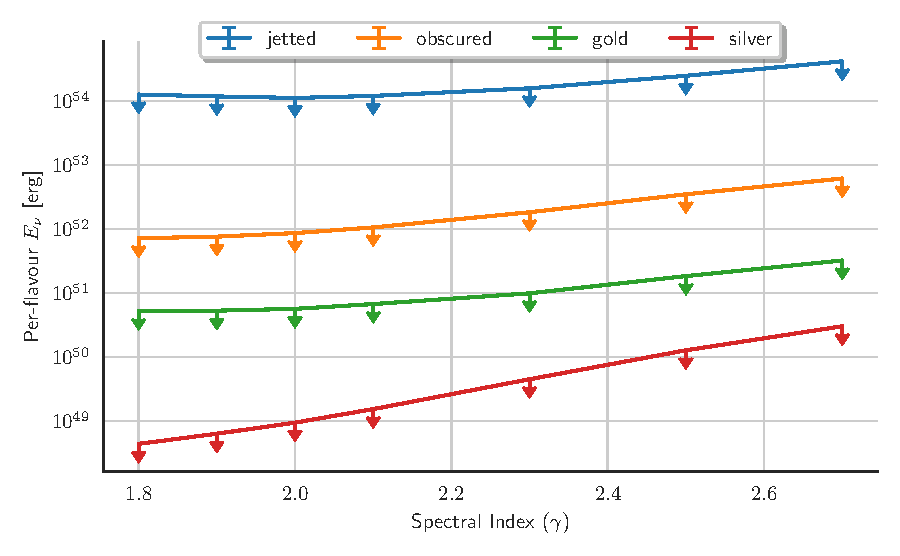
\includegraphics{results/catalogue_limits}
	\caption{Limits on the per-source neutrino emission for each catalogue.}
	\label{fig:cat_upper_limit}
\end{figure}

\subsection*{Population limits}

While the limits presented above constrain the contribution of those catalogues tested, we ultimately wish to constrain neutrino emission for the TDE population as a whole. If we \emph{assume that catalogue sources are representative of the broader population}, we can extrapolate from our per-source standard candle limits in Figure \ref{fig:cat_upper_limit} to the population flux. We seek to constrain the flux of two populations, namely jetted and non-jetted TDEs. For the latter case, we rely on the results of the golden TDE catalogue, because this sample is unlikely to be substantially contaminated by misclassified objects.

Using the most recent IceCube global fit of the astrophysical neutrino flux \sidecite{ic_global_fit_15}, with a best-fit spectrum of $E^{-2.50}$, we follow the procedure outline in Chapter \ref{ch:neutrino_cosmology}. We combine the golden TDE per-source limit shown in Figure \ref{fig:cat_upper_limit}, with a central local rate of $8 \times 10^{-7}$ Mpc$^{-3}$ year$^{-1}$ \sidecite{2018ApJ...852...72V} and a TDE source evolution \sidecite{Sun:2015bda} parameterised as:

\begin{equation}
\rho(z) \propto \left( (1 + z)^{-0.4} + \left( \frac{1 + z}{1.43} \right)^{6.4} +
\left( \frac{1 + z}{2.66} \right)^{14}
\right)^{-\frac{1}{2}}
\label{eq:tde_evolution}
\end{equation}

With this evolution, we constrain the contribution of non-jetted TDEs to be less than 25.3\% of the total. For jetted TDEs, under the assumption that they follow the same underlying source evolution in Equation \ref{eq:tde_evolution} with a central rate of $3 \times 10^{-11}$ Mpc$^{-3}$ year$^{-1}$ \cite{Sun:2015bda}, we find that they must contribute less than 1.3\% of the total.  These constraints are illustrated in Figure \ref{fig:DiffuseFlux}. 

\begin{figure}[!ht]
	\centering 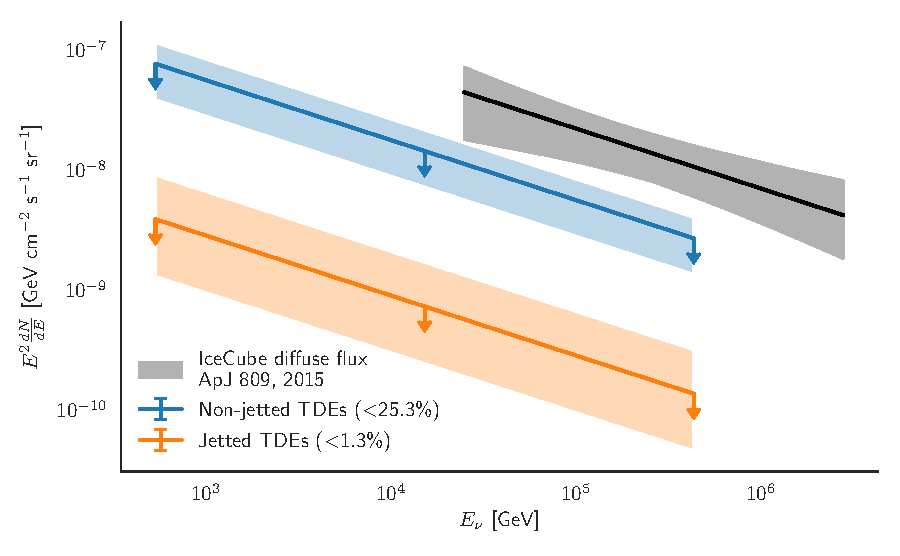
\includegraphics{results/tde_limits}
	\caption{Limits on the contribution of jetted and non-jetted TDEs to the diffuse neutrino flux.}
	\label{fig:DiffuseFlux}
\end{figure}

As the contribution from a population is directly proportional to the local population rate, the shaded bands indicate the uncertainty in our limits arising from rate estimates. For TDEs, these rates are a large source of uncertainty in neutrino flux. It will require systematic evaluation of observed TDE rates to enable more precise limits on neutrino emission. Propagating through the current local rate uncertainty, we constrain non-jetted TDEs to be less than 12.7\% - 38.0\%, and jetted TDEs to be less than 0.4\% - 3.0\% of the total. With a more precise future measurement of the local TDE rate, these values can be linearly rescaled to provide more accurate limits.

Such limits also critically depend on the source evolution of TDEs as a function of redshift, but this is not strongly constrained observationally because TDEs detections are generally confined to the local universe (z $\lesssim$ 0.3). Estimates are made primarily based on theoretical predictions derived from the rate of supermassive black holes (see Chapter \ref{ch:neutrino_cosmology}) \cite{Sun:2015bda}. We can instead consider a source evolution similar to the Star Formation Rate (SFR) \sidecite{sfr_madau_14}, parameterised as:

\begin{equation}
\rho(z) \propto\frac{(1+z)^{2.7}}{1 + ((1+z)/2.9)^{5.6}}
\label{eq:sfr_evolution}
\end{equation}

With Equation \ref{eq:sfr_evolution}, we would then find limits of 108.3\% (54.2\% - 162.5\%) for non-jetted TDEs and 5.5 \% (1.8\% - 12.8\%) for jettted TDEs. These limits are shown in Figure \ref{fig:DiffuseFluxSFR}. For such a scenario, the contribution of unresolved non-jetted TDEs is so large that the measured flux itself provides a stricter constraint than the catalogue test. However, even in that extreme scenario, the contribution of jetted TDEs to the diffuse neutrino flux remains subdominant.

\begin{figure}[!ht]
	\centering 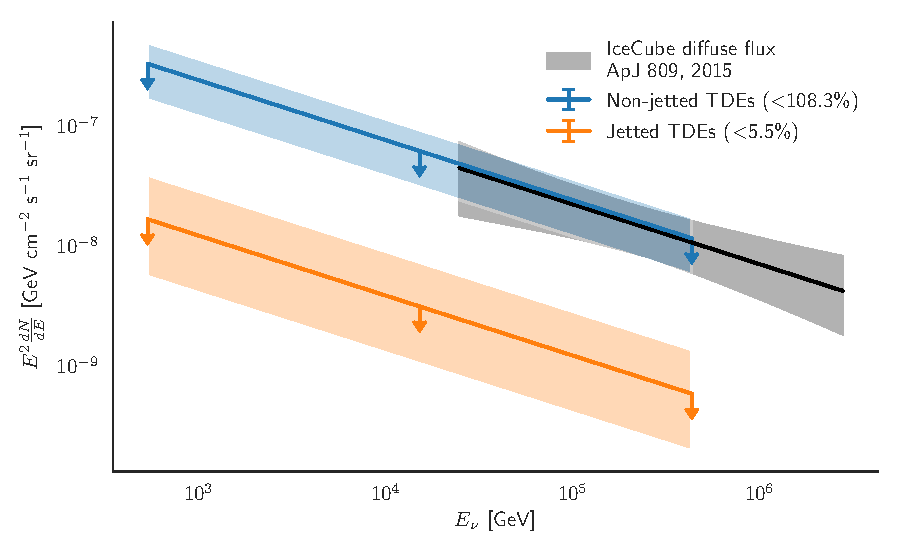
\includegraphics{results/tde_limits_sfr}
	\caption{Limits on the contribution of jetted and non-jetted TDEs to the diffuse neutrino flux, under the assumption of a source evolution proportional to the Star Formation Rate.}
	\label{fig:DiffuseFluxSFR}
\end{figure}

\subsection*{Individual TDEs}

In addition to the stacking analysis, four TDEs were selected for individual analysis. Two of the three jetted TDEs, Swift J1644+57 and Swift J2058+05, were chosen due to their luminosity, as well as their position in the northern hemisphere where IceCube has the highest effective area. In addition, ASSASN-14li and  XMMSL1 J0740-85 were chosen as non-jetted TDEs which were both nearby and bright. These four TDEs were the only catalogue sources that were also detected in radio observations, typically a tracer for relativistic particle acceleration. For each of the four individual TDEs, searches were conducted for neutrino clustering in both time and space, following the procedure outlined in Section \ref{sec:cluster_algorithm}. All single-object tests are described in Table \ref{tab:single_tests}.

\begin{table*}[]
	\centering
	\begin{tabular}{||c |c c c c | c c c c| c||} 
	\hline
	Source & R.A & Dec & T$_{0}$ & T$_{1}$ & n$_{s}$ & $\gamma$ & t$_{s}$ & t$_{e}$ & TS\\
	& (deg.) & (deg.) & (MJD) & (MJD) & & & (MJD) & (MJD) & \\
	\hline
	Swift J1644+57 & 251.21 & 57.58 & 55644.00 & 55749.00 & 0.68 & 1.98 & 55650.90 & 55746.25 & 0.06\\
	Swift J2058+05 & 314.58 & 5.23 & 55694.00 & 55798.00 & 2.78 & 4.00 & 55774.25 & 55780.00 & 2.28\\
	ASASSN-14li & 192.06 & 17.77 & 56851.00 & 57072.00 & 2.95 & 2.53 & 57022.68 & 57032.75 & 1.52\\
	XMMSL1 J0740-85 & 115.03 & 85.66 & 56718.00 & 56848.00 & 2.84 & 2.19 & 56806.95 & 56807.51 & 3.49\\
	\hline
	AT2018cow & 244.00 & 22.27 & 58256.90 & 58386.90 & 5.91 & 2.98 & 58283.83 & 58298.53 & 3.91\\
	\hline
	\end{tabular}
	\caption{Summary of the five individual TDEs for which the temporal-cluster-search method was applied. All but AT2018cow were included in the stacking analysis.}
	\label{tab:single_tests}
\end{table*}{}

The results of each fit are provided in Table \ref{tab:single_tests}, alongside pre-trial p-values. No significant emission was identified, and no discovery is claimed. Instead, upper limits are derived on neutrino emission for each source. As described in Section \ref{sec:cluster_algorithm}, the cluster-search method is more sensitive to shorter-scale emission. Upper limits were derived under the conservative assumption that neutrino emission was distributed uniformly in the search window, with any emission on shorter timescales being more constrained. 

\section{AT2018cow and FBOTs}

Following the four stacking analyses and four cluster-search analyses described above, an additional analysis was later performed on AT2018cow \sidecite{Margutti:2018rri}, a transient first discovered in 2018. It is now thought that AT2018cow was a nearby example of the recently-identified population known as ``Fast Blue Optical Transients" (FBOTs) introduced in Chapter \ref{ch:sources}. 

However, at the time of discovery, AT2018cow was initially thought to be a bright Broad-Lined type Ic (Ic-BL) supernova, and thus a member of the rare subclass associated with long GRBs and relativistic jets \sidecite{sn_grb_06}. As outlined in Chapter \ref{ch:sources}, many models predict that such SNe may be neutrino sources, so an IceCube \emph{Fast Response Analysis} was run on AT2018cow shortly after discovery \sidecite{ic_fra}. The IceCube search targeted choked-jet neutrino emission, and thus covered the 3-day period from the last non-detection to the first detection, aiming to isolate the supernova explosion time at which the neutrino emission would be expected. Ultimately, an excess of neutrinos was found in this time period, with a significance of 1.8 $\sigma$ \sidecite{2018ATel11785....1B}. The excess itself consisted of two signal-like neutrinos, which were considered significant owing to the small expected background for such a short search window.

Later multi-wavelength observations of AT2018cow were not consistent with a traditional Ic-BL SN, and the transient was later identified as a nearby example of an FBOT \sidecite{Perley:2018oky}. The exact nature of these FBOTs had been difficult to probe, since they were primarily discovered at high redshift \sidecite{drout_fbot}, but promptly-identified AT2018cow at 60 Mpc provided a rich multi-wavelength dataset. It has since been variously interpreted as a TDE with an Intermediate-Mass Black Hole, an extreme supernova or a Magnetar . In light of these developments, AT2018cow was re-analysed by the author in the context of a potential TDE classification. As for the other four individual TDEs detailed above, a dedicated search for neutrino clustering on timescales up to 130 days, extending from 30 days before peak to 100 days afterwards, was undertaken.  For this purpose, an additional year of IceCube data extending to October 2018 was analysed.

In this analysis of AT2018cow, a small excess was again found. Although the best-fit cluster from this search included the two signal-like neutrinos from the original IceCube analysis, when accounting for the expected fluctuations arising from background over the much longer 130 day search window, the significance of the excess was just 0.5 $\sigma$. The result is thus entirely consistent with expectations from atmospheric background, while not contradicting the original result published at the time. As such, no discovery is claimed and upper limits for AT2018cow are accordingly derived (illustrated in Figure \ref{fig:at2018cow_limits}). Though AT2018cow was not included in the catalogues when the stacking analysis was performed, it would naturally belong to the silver non-jetted TDE sample. 

\begin{figure}[!ht]
	\centering 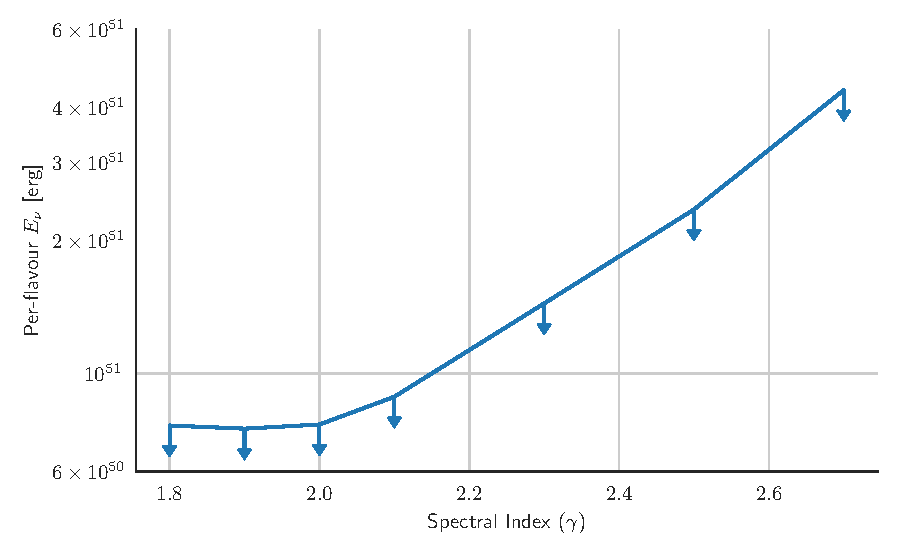
\includegraphics{results/at2018cow_limits}
	\caption{Limits on neutrino emission from AT2018cow, as a function of spectral index.}
	\label{fig:at2018cow_limits}
\end{figure}

The analysis of AT2018cow is the first example of a test for neutrino emission from FBOTs. In the time since discovery in 2018, there have been theoretical studies considering possible neutrino emission from FBOTs in general, and AT2018cow in particular \sidecite{fang_fbot_19}. The predicted neutrino emission is typically several orders of magnitude below the limits presented in Figure \ref{fig:at2018cow_limits}, and thus further supports the likely atmospheric origin for the neutrino excess \cite{2018ATel11785....1B}.

However, given that AT2018cow is by far the closest example of an FBOT, we can already consider the implications for the broader FBOT population emission. While initial estimates suggested that these objects might equal $\sim$4-7\% of the CCSN rate \cite{drout_fbot, fang_fbot_19}, these estimates have been superseded by results from magnitude-limited surveys such as ZTF, where a lack of additional FBOTs strongly suggest that the local rate must be $\sim$ 0.1\% of the CCSN rate \sidecite{ho_21}. 

Following the same procedure for TDEs, we find that FBOTs contribute less than 16\% of the total diffuse neutrino flux \emph{assuming that AT2018cow is representative of the broader FBOT population}. This further assumes a CCSN-like source evolution \sidecite{sfr_madau_14}, proportional to the star formation rate, and a local FBOT rate of 4 $\times$ 10$^{-7}$ Mpc$^{-3}$ yr$^{-1}$ \cite{ho_koala}. These limits are agnostic to the exact nature of FBOTs, whether they are a distinct population or a rare subgroup of some broader object class. In any case, it is clear  that any contribution of FBOTs to the diffuse neutrino flux must be subdominant.

\begin{figure}[!ht]
	\centering 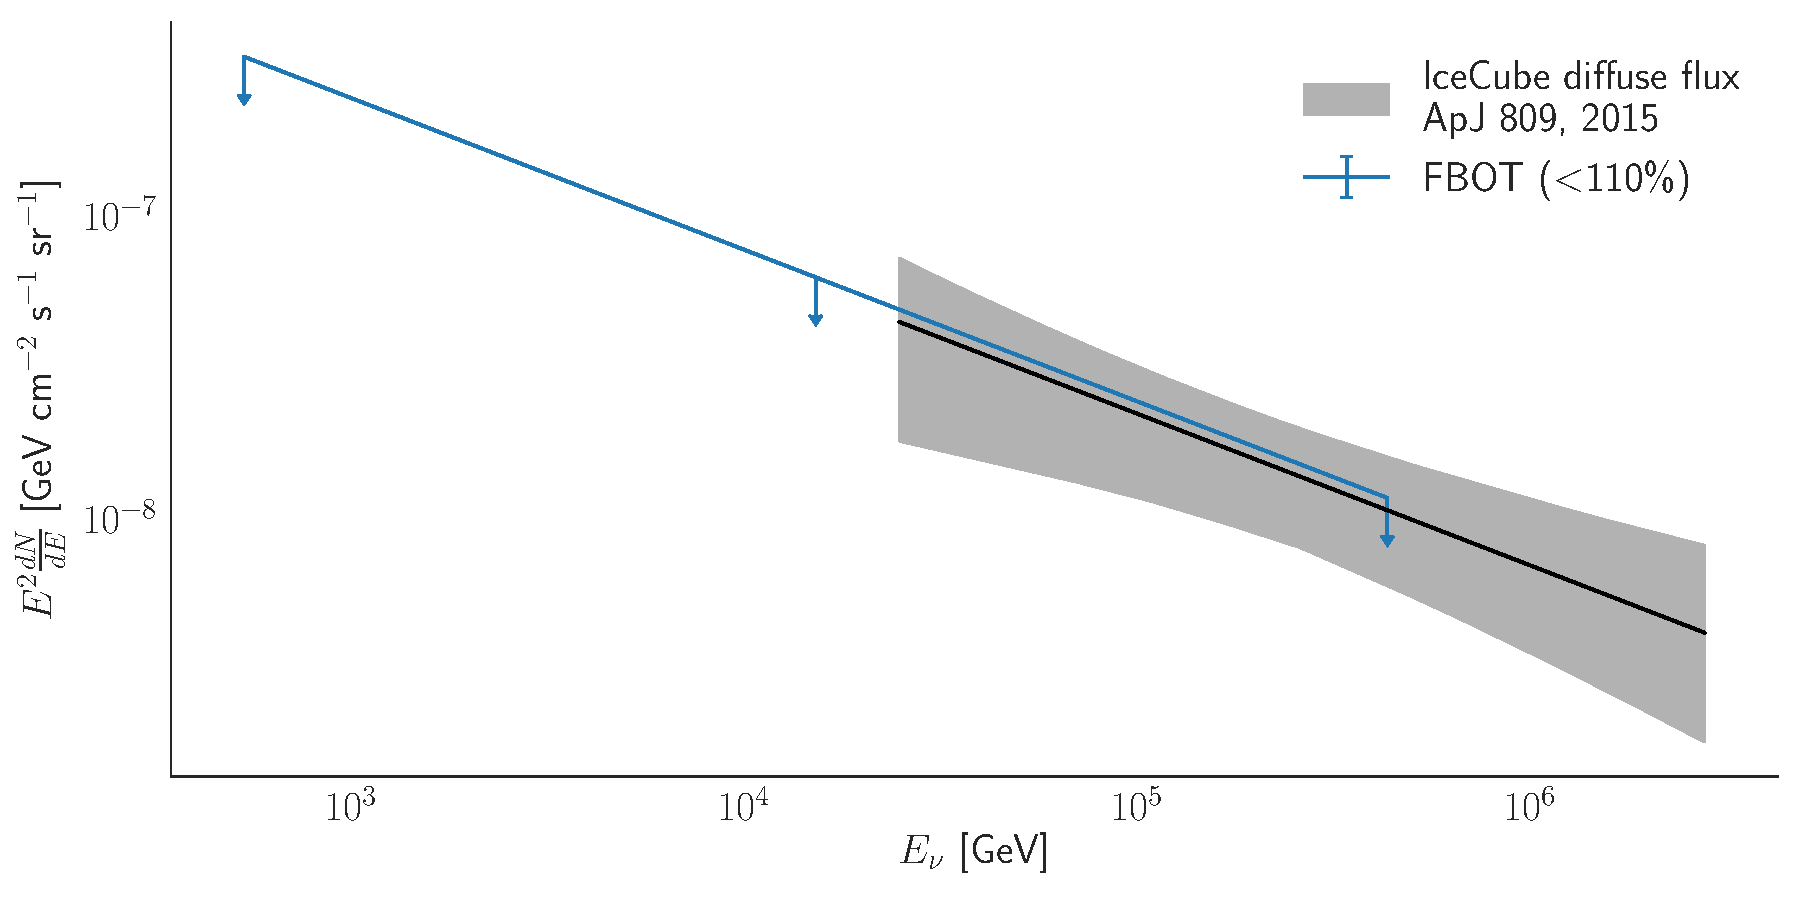
\includegraphics{results/fbot_limits}
	\caption{Limits on neutrino emission from FBOTs, using the limits from AT2018cow under the assumption of neutrino standard candles.}
	\label{fig:fbot_limits}
\end{figure}

\section{Robustness of Limits}

One key additional point is how robust the derived constraints are, given the many stated caveats. Full systematic studies are not typically re-performed for each individual IceCube neutrino source analysis \sidecite{ic_ps_10_yr}. This is due primarily to evidence from previous studies which demonstrated that the impact of systematic uncertainties on a typical Icecube neutrino point source search is O(\sim10\%), dominated by uncertainty on ice optical properties and DOM performance  \sidecite{ic_ps_7_yr}. This value is completely negligible in comparison to uncertainties on astrophysical population rates, as well as to additional uncertainties on the relative distribution of neutrinos across an astrophysical population. 

The searches introduced above are time-dependent analyses performed on specific windows, and are thus completely insensitive to any neutrino emission which may fall outside these windows. However, while the duration of neutrino emission may be uncertain for transients, it is expected that at least some substantial fraction of neutrino emission should occur during the periods of peak electromagnetic brightness. Thus the limits derived above can be extrapolated to cover neutrino emission models extending beyond the tested period. For example, if one predicts that only 50\% of neutrino emission from Jetted TDEs would occur in the first ~100 days, the population limit would be twice as high (2.6\% rather than 1.3\%) but still constraining.

A similar argument can be applied for deviations from an unbroken neutrino power law. For TDEs this would not be surprising, because the p$\gamma$ neutrino production models introduced in Chapter \ref{ch:sources} would instead favour a peaked neutrino spectrum. However, while the energy weightings illustrated in Figure \ref{fig:mc_dec_e} are based on different power laws, the likelihood analysis will detect excesses from any neutrino spectrum. If the signal follows the same energy distribution of the background, the energy term in the Point Source Likelihood (Equation \ref{eq:ps_llh}) will provide no discriminating power, but the analysis can still identify the corresponding spatial clustering. If instead there is some additional excess of neutrinos at either high or low energies, this can be well-approximated by a hard or soft neutrino power law respectively. Given that discoveries can be made with just 10-20 neutrinos, there is little power to discriminate between exact spectral shapes. 

\begin{figure}[!ht]
	\centering 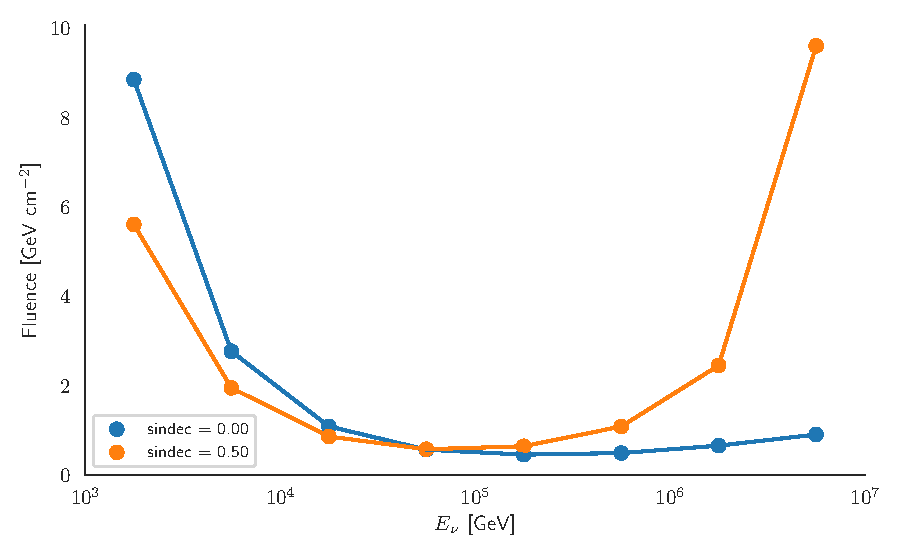
\includegraphics{results/energy_decades}
	\caption{Sensitivity of the Point Source Likelihood for a point source as a function of energy.}
	\label{fig:sens_disc_energy}
\end{figure}

However, as can be seen in Figure \ref{fig:cat_upper_limit_fluence}, the strength of the constraint depends on the general energy range at which neutrino emission is expected. This can be seen even more clearly in Figure \ref{fig:sens_disc_energy}, where the sensitivity is illustrated as a function of true neutrino energy. For a source at the horizon ($\sin(\delta)=0.0)$), in the range >10 TeV, the sensitivity does not vary by much, but is substantially worse at lower energies. For a more northern source ($\sin(\delta)=0.5)$), the sensitivity is similarly stable in the range $\sim$10 TeV - 1 PeV, above which it begins to degrade because of Earth absorption. This behaviour is in contrast to sources in the southern sky, for which the analysis is much less sensitive but improves with increasing energy. Within each tested catalogues, at least one of the five nearest sources lies at the horizon, and limits are generally dominated by such sources. We can thus state that all neutrinos emission scenarios between $\sim$10 TeV  and $\sim$1 PeV will be somewhat constrained by these results regardless of the exact energy spectrum, though clearly will be different for each individual model.

As was demonstrated for both TDEs and FBOTs, uncertainty on the properties of a given astrophysical population remains an important source of uncertainty in constraining the overall population neutrino emission. The local rate itself remains challenging to constrain particularly for rare transient classes such as jetted TDEs or FBOTs, though wide-field time-domain surveys such as ZTF and LSST should lead to continuing improvements in precision. Constraining the rate evolution is more challenging, particularly because even deep surveys such as LSST will not probe transient rates at very high redshift where much of the neutrino emission is expected. Ultimately this source of uncertainty will likely continue to dominate limits even with next-generation neutrino detectors and transient surveys.